% $Id$
\section{Neutrinoless double beta decay experiments}
\label{sec:gerda:nonubb}

\subsection{Sensitivity}
\label{sec:gerda:sensi}
The number of observed $0\nu\beta\beta$ decay events $N_{s}$ within the measuring time $t$, can be calculated as
\begin{equation}
  \label{eq:gerda:ns}
  N_{s} = M \cdot \kappa \cdot \frac{N_{A}}{M_{A}} \cdot \epsilon \cdot (1 - e^{-t/\tau}) \approx M \cdot \kappa \cdot \frac{N_{A}}{M_{A}} \cdot \epsilon \cdot \frac{t}{\tau},
\end{equation}
where, $M$ is the total mass of the source material, $\kappa$ is the mass fraction of the isotope under study, $N_{A}$ is Advogadro's number, $M_{A}$ is the atomic mass of the isotope, $\epsilon$ is the signal detecting efficiency, and $\tau$ is the mean lifetime of the decay. Since the measuring time $t$ is much shorter than the mean lifetime $\tau$, $(1 - e^{-t/\tau})$ is approximately to be $t/\tau$. The half lifetime, $T^{0\nu}_{1/2}$, is then
\begin{equation}
  \label{eq:gerda:thalf}
  T^{0\nu}_{1/2} = \ln2 \cdot \tau \approx \ln2 \cdot M \cdot \kappa \cdot \frac{N_{A}}{M_{A}} \cdot \epsilon \cdot \frac{t}{N_{s}}.
\end{equation}
The number of background events within the same time $t$, and within the energy window of interest $\Delta E$, is 
\begin{equation}
  \label{eq:gerda:nb}
  N_{b} = b \cdot M \cdot t \cdot \Delta E,
\end{equation}
assuming the background level of $b$ events per kilogram of source material per measuring year and per keV. If $N_{s}$ is smaller than the standard deviation of $N_{b}$, \textit{i.e.} $N_{s}<\sqrt{N_{b}}$, they would be regarded as the fluctuation of $N_{b}$ with high possibility. In this case the relation
\begin{equation}
  \label{eq:gerda:thalfb}
  T^{0\nu}_{1/2} > \ln2 \cdot M \cdot \kappa \cdot \frac{N_{A}}{M_{A}} \cdot \epsilon \cdot \frac{t}{\sqrt{N_{b}}} = \ln2 \cdot \kappa \cdot \frac{N_{A}}{M_{A}} \cdot \epsilon \sqrt{\frac{M t}{b \Delta E}}
\end{equation}
can be used to set a lower limit on the half lifetime. Combined with eq.~\ref{eq:0nurate}, the following relation can be deduced to set a upper limit on the effective Majorana neutrino mass:
\begin{equation}
  \label{eq:gerda:mbb}
  m_{\beta\beta} < \sqrt{\frac{M_{A}}{\ln2 \cdot \kappa \cdot N_{A} \cdot \epsilon}} \sqrt{\frac{1}{G_{0\nu}(Q,Z)}} \frac{1}{|\mathcal{M}_{0\nu}|} (\frac{b \Delta E}{M t})^{1/4}
\end{equation}
This relation can be used to estimate the sensitivity of a $0\nu\beta\beta$ decay experiment. A dedicated analysis can be found in Ref.~\cite{Cal06}. The left plot in Fig.~\ref{fig:gerda:limit} taken from Ref.~\cite{Cal06} shows the expected 90\% probability lower limit on the half lifetime for $0\nu\beta\beta$ decay versus the exposure under different background conditions. Also shown is the half lifetime for the claimed observation by H. V. Klapdor-Kleingrothaus \textit{et al.}~\cite{Hei04}. The right plot shows the expected 90\% probability upper limit on the effective Majorana neutrino mass versus the exposure under different background conditions. The effective Majorana neutrino mass for the claimed observation is also shown. All mass values are determined from the half lifetime using the matrix element reported in Ref~\cite{Rod07}.
\begin{figure}[tbhp]
  \centering
  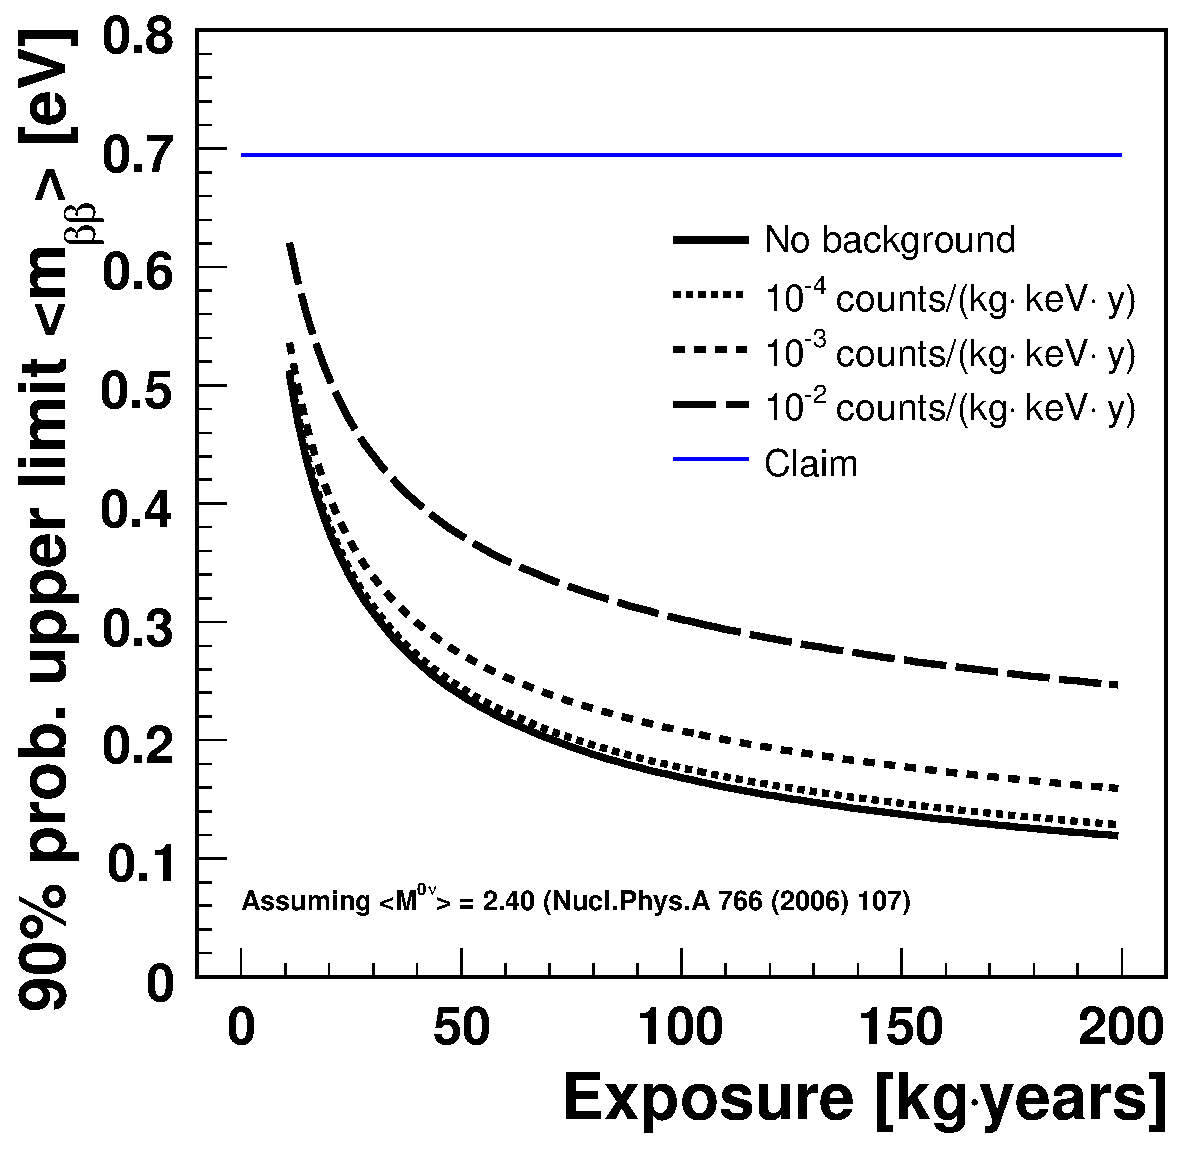
\includegraphics[width=0.4\textwidth]{limit_mass}  \hfil
  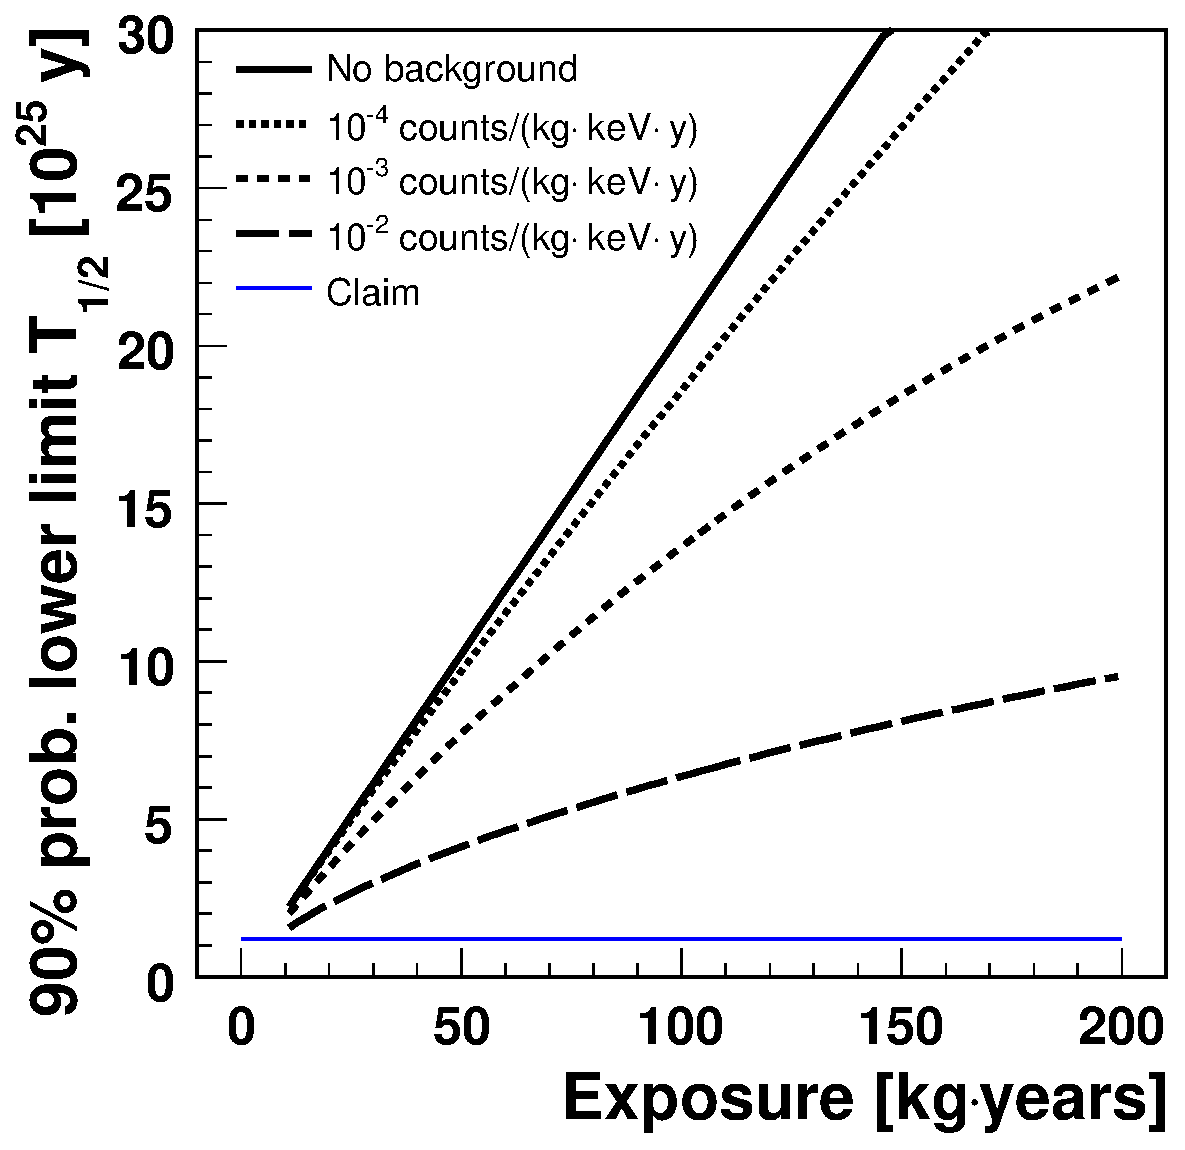
\includegraphics[width=0.4\textwidth]{limit_halflife}
  \caption{The expected 90\% probability lower limit on the half     lifetime for $0\nu\beta\beta$ decay (left) and the expected 90\%     probability upper limit on the effective Majorana neutrino mass     (right) versus the exposure under different background conditions.     Also shown is the half lifetime and the effective Majorana     neutrino mass for the claimed observation by H. V.     Klapdor-Kleingrothaus \textit{et al.}~\cite{Hei04}. All mass     values are determined from the half lifetime using the matrix     element reported in Ref~\cite{Rod07}.}
  \label{fig:gerda:limit}
\end{figure}

\subsection{General consideration}
\label{sec:gerda:gencon}
According to eq.~\ref{eq:gerda:mbb}, to design a $0\nu\beta\beta$ decay experiment with high sensitivity, \textit{i.e.} the capability to set a lower limit on $m_{\beta\beta}$, the following requirement needs to be fulfilled as much as possible:
\begin{itemize}
\item the source material $M$ should be as much as possible;
\item the natural abundance of the isotope under study should be large, or it is easy to enrich the isotope;
\item the calculation of the nuclear matrix element $|\mathcal{M}_{0\nu}|$ for this isotope should be accurate;
\item since $G_{0\nu}(Q,Z) \propto Q^{5}$, the $Q$-value should be large, and better to be larger than 2.6~MeV, in order to be above all the natural radioactive decay lines;
\item the signal detecting efficiency should be large;
\item the energy resolution should be good in order to have a small $\Delta E$;
\item last but not the least, the background level $b$ should be as low as possible.
\end{itemize}
After all, one needs to wait until a better upper limit on $T^{0\nu}_{1/2}$ could be set or an observation could be claimed.

Except for background suppression techniques, the experimental approach would be mostly determined by the choice of the source material. Table~\ref{tab:gerda:iso} presents a selection of isotopes used or planned to be used to search $0\nu\beta\beta$ decay. Also listed are their $Q$-values, nuclear matrix elements~\cite{Mut90, Rod07, Sim08, Cau08}, natural abundance $\kappa$ and properties important for the experimental design. Different experimental approaches can be classified into two categories: 1. the source material can be used to produce the detector; 2. the source is not the detector, the decay products need to be detected using equipment around the source.
\begin{table}[htbp]
  \centering
  \caption{A selection of possible source candidates for         $0\nu\beta\beta$ decay experiments. Also listed are their $Q$-values,     nuclear matrix elements, natural abundance $\kappa$ and properties     important for the experimental design.}
  \label{tab:gerda:iso}
  \begin{minipage}{\linewidth}
    \begin{tabular}{ccccc} \hline Isotope & $Q$ [MeV] &       $\mathcal{M}_{0\nu}$ & $\kappa$ [\%] & Properties \\\hline       $^{48}$Ca & 4.271 & 0.67\footnote{The values are from the ISM         (Interacting Shell Model) calculation~\cite{Cau08}.  The other         $\mathcal{M}_{0\nu}$ values with errors are from the QRPA         (Quasi-particle Random Phase Approximation)         calculations~\cite{Rod07}. The errors are from the measurement         of $2\nu\beta\beta$ experiments.} & 0.19 & CaF2 is       scintillator \\
      $^{76}$Ge & 2.039 & $4.51 \pm 0.17$ & 7.8 & semiconductor \\
      $^{82}$Se & 2.995 & $4.02 \pm 0.15$ & 9.2 & - \\
      $^{96}$Zr & 3.350 & $1.12 \pm 0.03$ & 2.8 & - \\
      $^{100}$Mo & 3.034 & $3.34 \pm 0.19$ & 9.6 & - \\
      $^{116}$Cd & 2.809 & $2.74 \pm 0.19$ & 7.5 &       CdZnTe\footnote{There are more than one isotope in the CdZnTe         crystal that could undergo $0\nu\beta\beta$ decay. The rest of         them are $^{70}$Zn with $Q = 1.001$~MeV, $\kappa = 0.62\%$,         $^{114}$Cd with $Q = 0.534$~MeV, $\kappa = 28.7\%$, $^{128}$Te         with $Q = 0.868$~MeV, $\kappa = 31.7\%$ and $^{130}$Te.} is       room temperature semiconductor\\
      $^{124}$Sn & 2.287 & $2.11^{a}$ & 5.8 & semiconductor \\
      $^{130}$Te & 2.530 & $3.26 \pm 0.12$ & 35 & TeO$_{2}$ can be       used as bolometer\\
      $^{136}$Xe & 2.480 & $2.11 \pm 0.11$ & 8.9 & filling gas of       time drift       chamber\\
      $^{150}$Nd & 3.367 & $4.74 \pm 0.20$ & 5.6 & neodymium solution       is liquid       scintillator\\
    \end{tabular}
  \end{minipage}
\end{table}

\subsection{Source is detector}
\label{sec:gerda:sed}
As shown in Table~\ref{tab:gerda:iso}, quit a few $0\nu\beta\beta$ decay candidates have special properties which allow them to be used as detectors as the same time.


\subsection{Source is not  detector}
\label{sec:gerda:sued}

\section{The GERDA experiment}
\label{sec:gerda:concept}

\subsection{Concept}
\label{sec:gerda:concept}

\subsection{Status}
\label{sec:gerda:status}


%%% Local Variables:
%%% mode:latex
%%% TeX-master: "thesis"
%%% End:
